% ═════════════════════════════════════════════════════════════════════════════
% Chapter 9: Design and Modeling of LEON
% ═════════════════════════════════════════════════════════════════════════════

\chapter{Design and Modeling of LEON}
\label{chap:design}

% ═════════════════════════════════════════════════════════════════════════════
\section{\textcolor[HTML]{0066CC}{Design Objectives}}
\label{sec:design-objectives}
% ═════════════════════════════════════════════════════════════════════════════

The design of LEON is grounded on four strategic pillars:

\begin{enumerate}
    \item \textcolor[HTML]{003D99}{\textbf{Conversational Flexibility}} : the conversational interface (Copilot Studio) must allow users to navigate freely among services (Who-is-Who, Gate tracking, Workload management) without imposing rigid flow, while guiding toward relevant actions.
    
    \item \textcolor[HTML]{003D99}{\textbf{Validation Determinism}} : the SpecValidator block must apply deterministic and reproducible validation rules, independent of the conversational layer, ensuring consistency in specification assessments.
    
    \item \textcolor[HTML]{003D99}{\textbf{Transparent Integration}} : LEON must integrate seamlessly with Stellantis's existing systems via enterprise connectors (directories, storage) and APIs, without disrupting current workflows.
    
    \item \textcolor[HTML]{003D99}{\textbf{Traceability and Audit}} : every action performed (search, modification, validation, notification) must be recorded to ensure compliance, auditability, and anomaly resolution. The system must maintain a complete history of decisions and modifications.
\end{enumerate}

% ═════════════════════════════════════════════════════════════════════════════
\section{\textcolor[HTML]{0066CC}{Functional View}}
\label{sec:design-functional-view}
% ═════════════════════════════════════════════════════════════════════════════
This section gives a description of the LEON system from the functional point of view. It gives details about services provided to the user and some system/actor interactions. The behavior of the system is described from user point of view, without technical constraints.
\subsection{Primary Services}

LEON delivers two categories of services:

\vspace{0.2cm}
\noindent\textcolor[HTML]{0066CC}{\textbf{A) Governance Services}}
Accessible via conversation, these services enable users to:
\begin{itemize}
    \item \textcolor[HTML]{003D99}{\textbf{Search for responsible party}} : query the Who-is-Who database to identify the person responsible for a component in a project.
    \item \textcolor[HTML]{003D99}{\textbf{Retrieve gate status}} : obtain current status (Gate 1, Gate 2, Gate 3, or other states defined by Stellantis).
    \item \textcolor[HTML]{003D99}{\textbf{Update responsibility assignments}} : modify responsibility assignments (subject to access control).
    \item \textcolor[HTML]{003D99}{\textbf{Manage workload}} : view and create/update task assignments and resource availability.
    \item \textcolor[HTML]{003D99}{\textbf{Send notifications}} : trigger communications (emails, reminders) to targeted stakeholders.
    \item \textcolor[HTML]{003D99}{\textbf{Upload deliverables}} : upload a file to the correct location associated with a gate.
\end{itemize}
\vspace{-4pt}

\vspace{0.2cm}
\noindent\textcolor[HTML]{0066CC}{\textbf{B) Validation Service}}
The SpecValidator service ensures that the technical specification complies with the engineering rules. It is invoked via conversational interface on user‘s request for the specification check.
\begin{itemize}
    \item \textcolor[HTML]{003D99}{\textbf{Specification templates and Rule files}} : The process of validation is relying on several structured inputs like references templates and set of rules that specify the content and quality of a specification then the service validates the document systematically.
    \item \textcolor[HTML]{003D99}{\textbf{Output}} :The validation output is provided as an organized report showing compliance results, non-compliance observations and proposed corrections. The report permits to display results to user and keeps document unchanged.
\end{itemize}
\vspace{-4pt}

\subsection*{\textcolor[HTML]{003D99}{Use Case Diagram}}

Figure~\ref{fig:leon-usecase-en} shows the use case diagram for the LEON system. This graph represents the relationship between the user and the system from a functional perspective.\\
The main users are engineer, project manager and administrators. The way they use the system is dependent on their level of control within the governance framework.
\vspace{-8pt}
\begin{figure}[H]
    \centering
    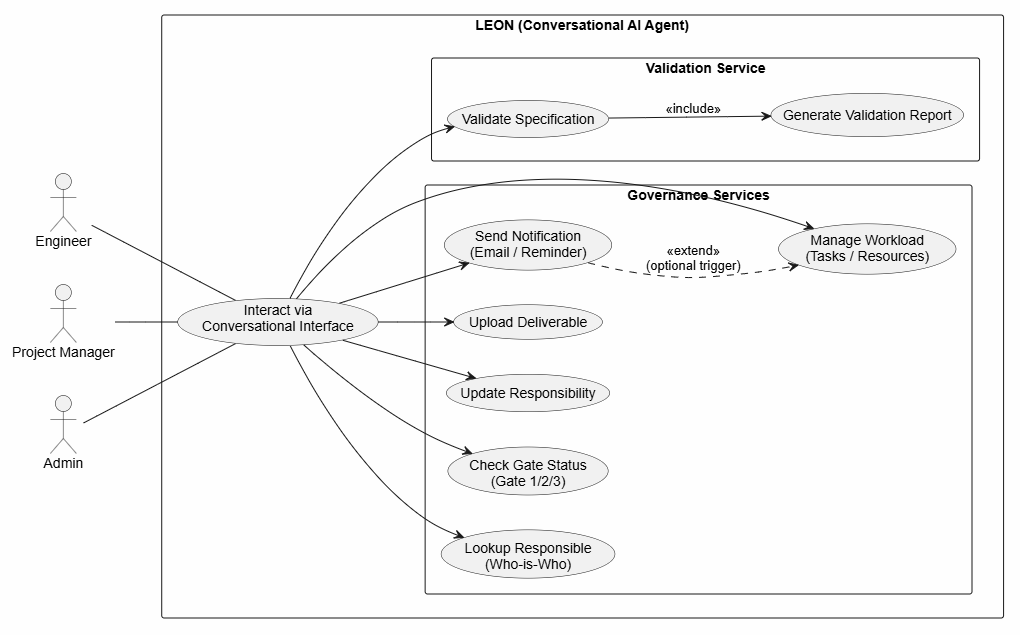
\includegraphics[width=0.85\textwidth]{images_pfe/use case diagram.png}
    \caption{LEON Use Case Diagram, high-level functional view}
    \label{fig:leon-usecase-en}
\end{figure}
\FloatBarrier
\vspace{-4pt}

These use cases are organized into two main groups, Services for Governance and Services for validation. The governance services covers governance related data (Who-is-Who, status of the Gate ownership) and data management (change of responsibility, document linking, document uploading) and services for Coordination (notifications, managing of training workflows). The validation services covers services for the SpecValidator module that checks technical specifications and generates technical reports about validation.\\
\vspace{0.5cm}
Centrally there is one conversational interface and therefore the services are accessed through one point of interaction, which makes switching between them simpler. In the diagram some connections are made between use cases; this is because of some inputs that need to be created (e.g. reports of validation) and some are dependent on others.\\
\vspace{0.5cm}
To conclude, in this functional view, LEON is perceived as a coherent layer among the set of governance functions and the set of distributed data.
% ═════════════════════════════════════════════════════════════════════════════
\section{\textcolor[HTML]{0066CC}{Structural View (Architecture)}}
\label{sec:design-structural-view}
% ═════════════════════════════════════════════════════════════════════════════

\subsection{Layered Architecture}

Under the layered architecture, this section will demonstrate the structural view of the LEON system in layered architecture form. It would be beneficial to separate the concern system of the user interface, the business, the data and the validation.

\vspace{0.2cm}
LEON is organized into four main logical layers:

\noindent\textcolor[HTML]{0066CC}{\textbf{1. Presentation / Conversation Layer}}
\begin{itemize}
    \item This represents the system entry layer. It provides the interaction with the user through a conversational user interface to enable stakeholders to access system services through a natural language.
    \item The described system is built on top of Copilot Studio that takes the users intentions and passes the request on to the corresponding service, furthermore it allows for conversational interactions.
    \item Role: Offers an interface that allows users to become abstract from applications, to interpret and validate their requests, and that is the interface to all appropriate services.
\end{itemize}

\noindent\textcolor[HTML]{0066CC}{\textbf{2. Orchestration and Business Logic Layer}}
\begin{itemize}
    \item This layer deals with performing all the operations related to the governance part. It receives commands from the Conversational Layer to be executed and then communicate with the interacting services.
    \item It implements governance functions (e.g. responsibility lookup, gate status retrieve, workload updates and message handling) using workflow features. It also handles the interface to external enterprise systems (e.g. directory services, document repositories and messaging).
    \item Role: Control the overall operations of the system and functionalities by defining the interaction flow among User, Data and Validation service
\end{itemize}

\noindent\textcolor[HTML]{0066CC}{\textbf{3. Processing / Validation Layer (Specialized)}}
\begin{itemize}
    \item This layer owns the processing units which are used to process domain-specific information. It is represented by the SpecValidator service in LEON, which checks the technical specifications.
    \item Validation is rule based and is executed using pre-defined templates from a repository which make validation a repeatable process. As validation is a singleton layer it doesn‘t depend on the conversational flow making validation activities deterministic.
    \item Role: Executes the task, separate validation logic from the UI.
\end{itemize}

\noindent\textcolor[HTML]{0066CC}{\textbf{4. Data and Configuration Layer}}
\begin{itemize}
    \item This layer contains the configuration data components as well as data components necessary for the system. Data components like the administration data sources (workloads, responsibilities etc) along with configuration components for validation exist in this layer.
    \item This Data is then archived in enterprise stores which might be document management systems or structured data stores. The system will also provide logging/auditing to achieve a clear trace of user/system interaction and to comply with standards.
    \item Role: provides long-term storage, configuration resources and ensures data integrity, consistency and traceability.
\end{itemize}

\subsection*{\textcolor[HTML]{003D99}{Architecture Diagram (Components)}}

\vspace{-8pt}
\begin{figure}[H]
    \centering
    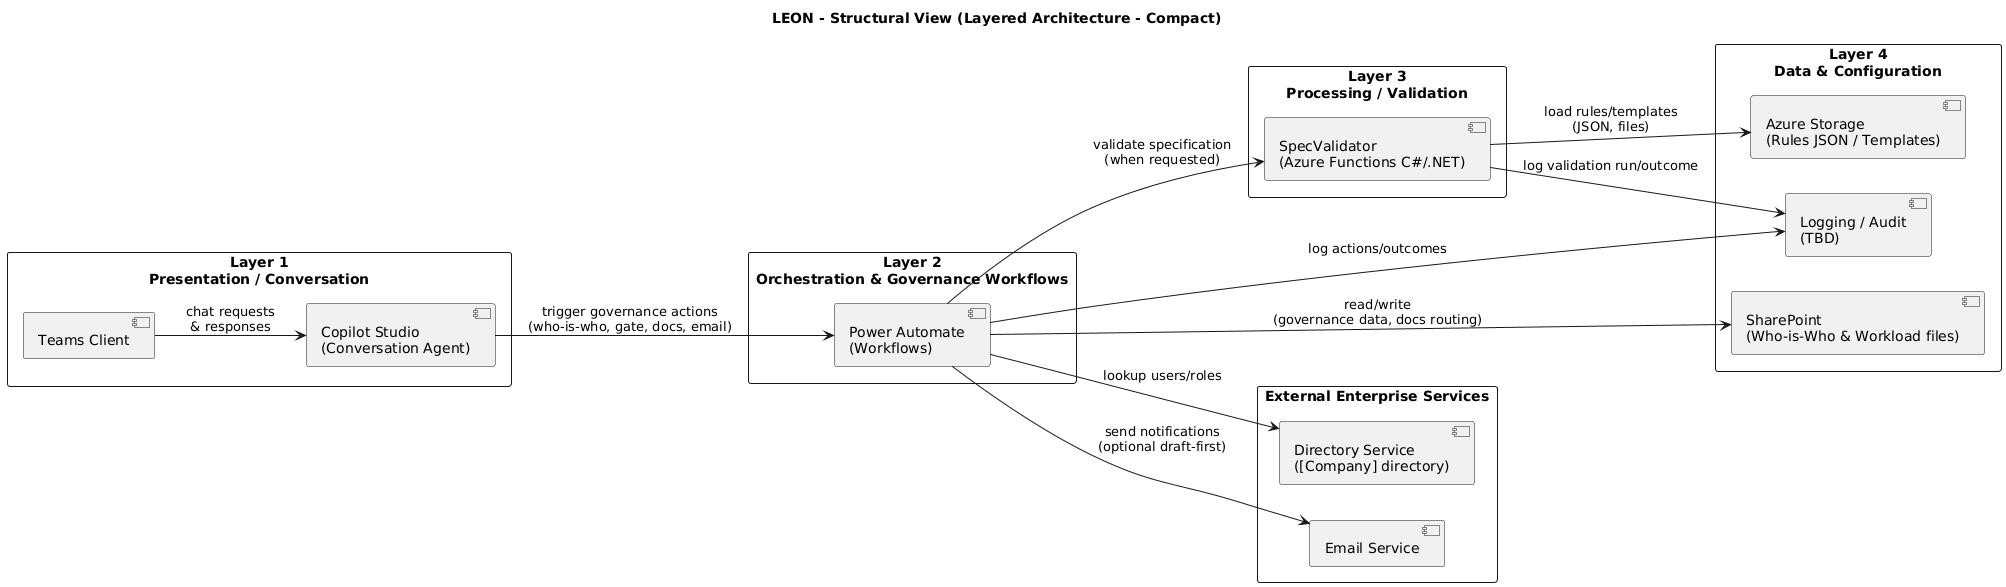
\includegraphics[width=0.9\textwidth]{images_pfe/structural view.png}
    \caption{Structural View: Architecture Diagram of LEON Components.}
    \label{fig:structural-view}
\end{figure}
\FloatBarrier
\vspace{-4pt}

The figure~\ref{fig:structural-view} presents the LEON architecture modeled according to the layers mentioned above. It highlights how the dialogue interface, orchestration capabilities, validation services and data sources interact with the activities related to governance.
% ═════════════════════════════════════════════════════════════════════════════
\section{\textcolor[HTML]{0066CC}{Dynamic View}}
\label{sec:design-dynamic-view}
% ═════════════════════════════════════════════════════════════════════════════

\subsection*{\textcolor[HTML]{003D99}{Primary Scenario: Specification Validation}}

Figure~\ref{fig:leon-sequence-en} shows the interaction sequence for specification validation in LEON.

\vspace{-8pt}
\begin{figure}[H]
    \centering
    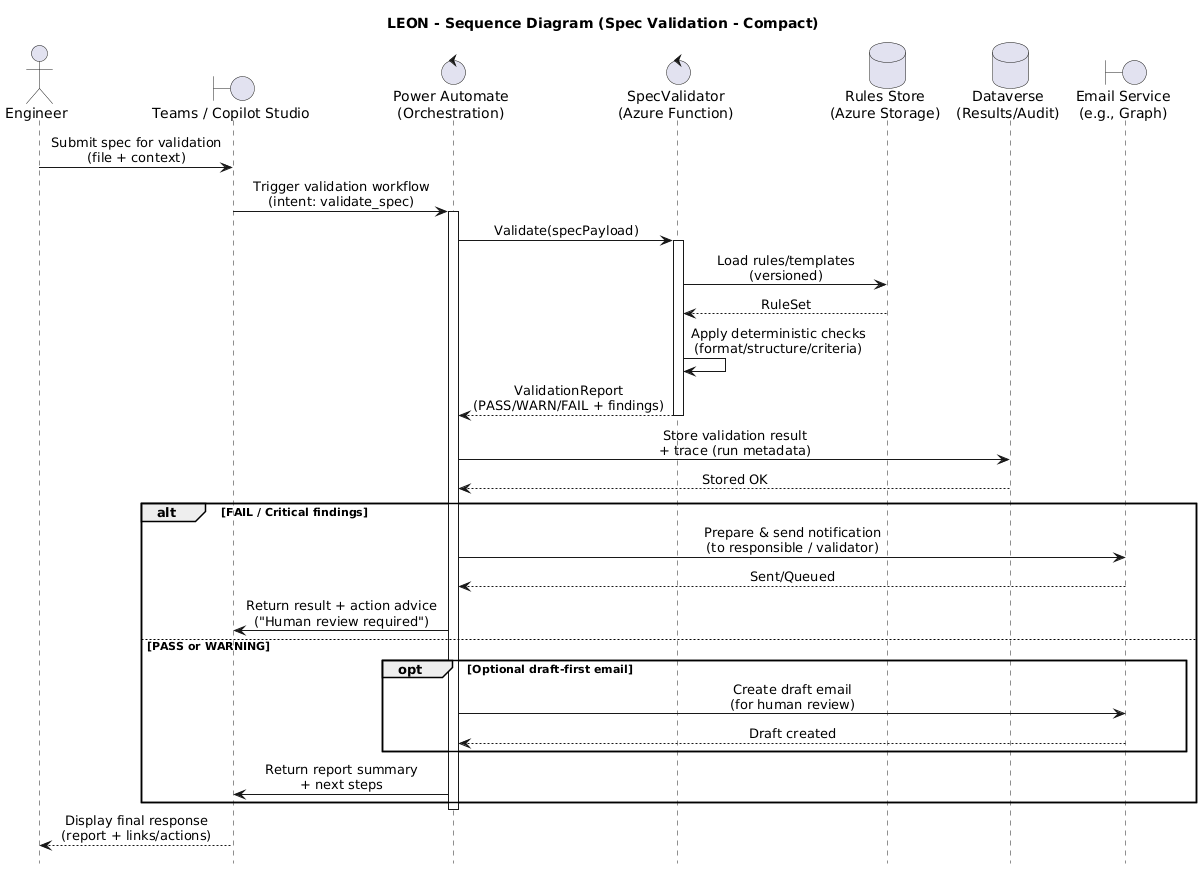
\includegraphics[width=0.9\textwidth]{images_pfe/sequence_diagram.png}
    \caption{UML Sequence Diagram: specification validation scenario showing interaction between Copilot Studio, Power Automate, SpecValidator, and Azure Storage.}
    \label{fig:leon-sequence-en}
\end{figure}
\FloatBarrier
\vspace{-4pt}

The sequence of events starts when the user inputs the specification in the conversational interface. The orchestration layer receives the entering specification request and starts the validation workflow.\\
The validation service receives the specification and uses a set of validation rules that is represented as a set of configuration information retrieved from the configuration layer. The result of validation is a formal validation report of the specification.\\
There are two execution flows according to the outcome. The critical problems would make the system execute other actions (e.g. notify interested people who should be responsible for that, request an expert review). The non-critical problem would make the system give back the overview of the validation with suggested action.\\
The result is then sent back to the user via the orchestration layer and is displayed through conversational interface.

% ═════════════════════════════════════════════════════════════════════════════
\section{\textcolor[HTML]{0066CC}{Data Model (Conceptual)}}
\label{sec:design-data-model}
% ═════════════════════════════════════════════════════════════════════════════

\subsection*{\textcolor[HTML]{003D99}{Key Conceptual Entities}}

Conceptual data model represents the core objects of the LEON governance process and the relations between these objects. It gives a high-level view on the structure of project data, responsibilities, validation and interaction.
\vspace{0.2cm}
\noindent\textcolor[HTML]{0066CC}{\textbf{Entities}}

\begin{description}
    \item[\texttt{Project}] A combination (in a folder) of components, deliverables and governance.
    
    \item[\texttt{Component}] Is the smallest logical and technical unit of a project. It can be tested, as one entity, and have a person or persons accountable.
    
    \item[\texttt{Actor/Responsible}] Human involved in governance, identified through the governance directory. A responsible may be a component owner or task owner.
    
    \item[\texttt{Gate}] Designates a stage in the project‘s life cycle (i.e. Gate 1, Gate 2, Gate 3) with specific validation needs and fields of competence
    
    \item[\texttt{Specification}] Technical document or deliverable of a component and a gate that can be validated.
    
    \item[\texttt{ValidationRule}] A preexisting rule providing the validation condition in accordance with specifications and context.
    
    \item[\texttt{Assignment}] assigning tasks to a person, considering his workload and scheduling constraints
    
    \item[\texttt{AuditLog}] The AuditLog object helps record what‘s being done within the system: what was doing it, who was doing it and when.
\end{description}

\subsection*{\textcolor[HTML]{003D99}{Primary Relationships}}

\begin{itemize}
    \item \textcolor[HTML]{003D99}{\textbf{Project} \texttt{1..N} \textbf{Component}} : a project contains multiple components.
    \item \textcolor[HTML]{003D99}{\textbf{Component} \texttt{1..N} \textbf{Responsible}} : a component may have multiple responsible parties (over time or by role).
    \item \textcolor[HTML]{003D99}{\textbf{Gate} \texttt{1..N} \textbf{ValidationRule}} : each gate is associated with a set of rules.
    \item \textcolor[HTML]{003D99}{\textbf{Specification} \texttt{N..1} \textbf{Gate}, \textbf{Component}} : each specification is linked to a Gate and Component.
    \item \textcolor[HTML]{003D99}{\textbf{Actor} \texttt{1..N} \textbf{Assignment}} : an actor may have multiple assignments.
    \item \textcolor[HTML]{003D99}{\textbf{AuditLog} \texttt{N..1} \textbf{Actor}} : each action is traced to the actor who performed it.
\end{itemize}

\subsection*{\textcolor[HTML]{003D99}{Conceptual Representation}}

\vspace{-8pt}
\begin{figure}[H]
    \centering
    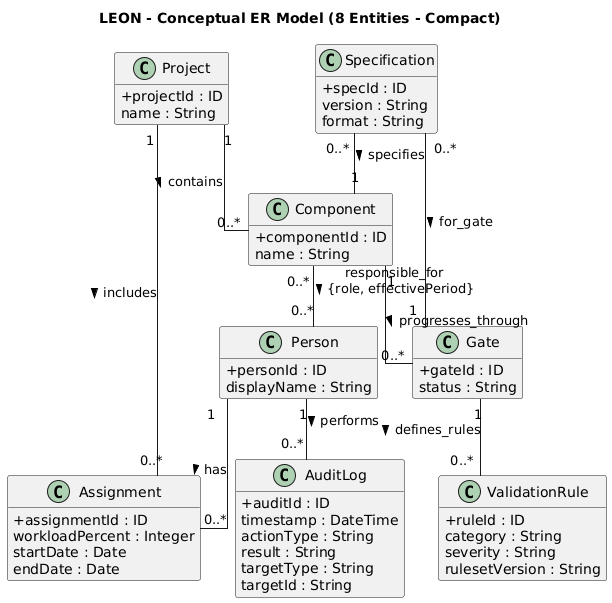
\includegraphics[width=0.9\textwidth]{images_pfe/conceptual ER.png}
    \caption{Conceptual Entity-Relationship Diagram of LEON.}
    \label{fig:conceptual-er}
\end{figure}
\FloatBarrier
\vspace{-4pt}
This diagram illustrates how the various components, the relation between entities and the governance data, the validation and system interaction are working together.


% ═════════════════════════════════════════════════════════════════════════════
\section{\textcolor[HTML]{0066CC}{V-Model: Design-to-Verification Traceability}}
\label{sec:design-vmodel}
% ═════════════════════════════════════════════════════════════════════════════
The V-Model (Verification \& Validation) establishes the complete traceability chain from design artifacts to verification evidence. Figure~\ref{fig:vmodel_leon} synthesizes:
\usetikzlibrary{positioning,arrows.meta,shapes.geometric}

\begin{figure}[H]
    \centering
    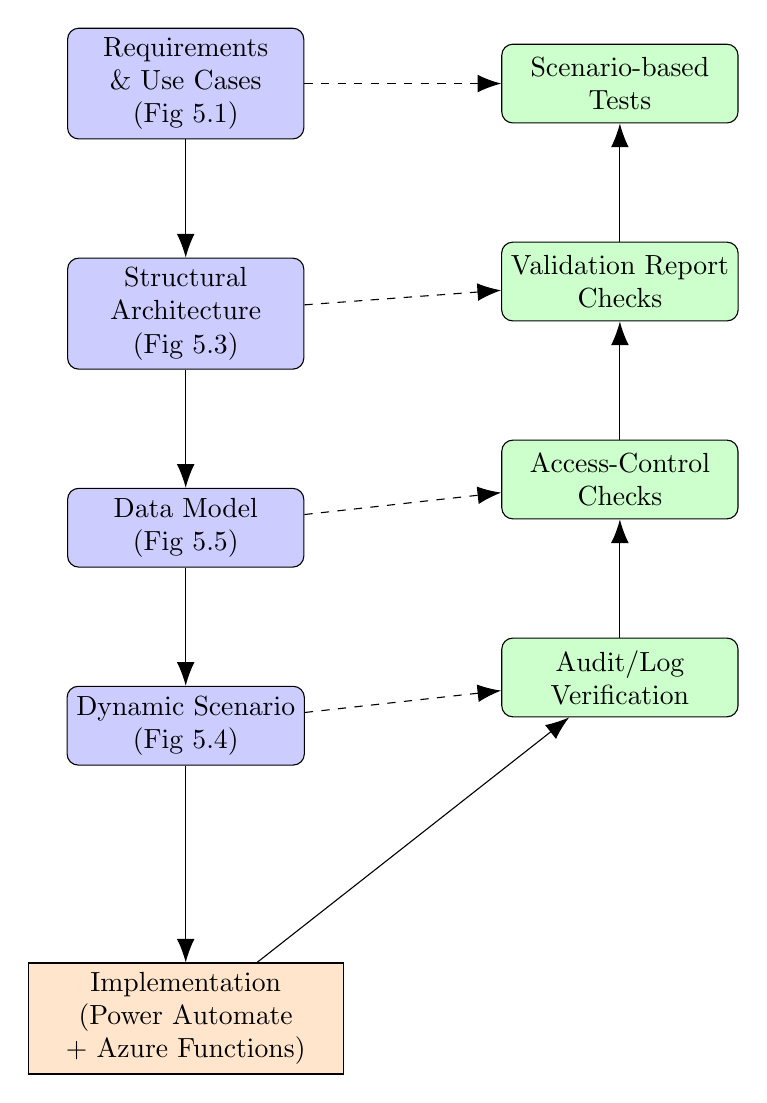
\begin{tikzpicture}[
        node distance=1.5cm and 2.5cm,
        every node/.style={align=center},
        artifact/.style={rectangle, draw, rounded corners, minimum width=3cm, minimum height=1cm, fill=blue!20},
        evidence/.style={rectangle, draw, rounded corners, minimum width=3cm, minimum height=1cm, fill=green!20},
        implementation/.style={rectangle, draw, minimum width=4cm, minimum height=1cm, fill=orange!20},
        trace/.style={dashed, -{Latex[length=3mm]}}
    ]

    % Left side (Definition/Design Artifacts)
    \node[artifact] (req) {Requirements \\ \& Use Cases \\ (Fig 5.1)};
    \node[artifact, below=of req] (arch) {Structural \\ Architecture \\ (Fig 5.3)};
    \node[artifact, below=of arch] (data) {Data Model \\ (Fig 5.5)};
    \node[artifact, below=of data] (dynamic) {Dynamic Scenario \\ (Fig 5.4)};

    % Bottom (Implementation)
    \node[implementation, below=of dynamic, yshift=-1cm] (impl) {Implementation \\ (Power Automate \\ + Azure Functions)};

    % Right side (Verification/Validation Evidence)
    \node[evidence, right=of req] (tests) {Scenario-based \\ Tests};
    \node[evidence, below=of tests] (validation) {Validation Report \\ Checks};
    \node[evidence, below=of validation] (access) {Access-Control \\ Checks};
    \node[evidence, below=of access] (audit) {Audit/Log \\ Verification};

    % Arrows (V-Model)
    \draw[-{Latex[length=3mm]}] (req) -- (arch);
    \draw[-{Latex[length=3mm]}] (arch) -- (data);
    \draw[-{Latex[length=3mm]}] (data) -- (dynamic);
    \draw[-{Latex[length=3mm]}] (dynamic) -- (impl);

    \draw[-{Latex[length=3mm]}] (impl) -- (audit);
    \draw[-{Latex[length=3mm]}] (audit) -- (access);
    \draw[-{Latex[length=3mm]}] (access) -- (validation);
    \draw[-{Latex[length=3mm]}] (validation) -- (tests);

    % Traceability Links
    \draw[trace] (req) -- (tests);
    \draw[trace] (arch) -- (validation);
    \draw[trace] (data) -- (access);
    \draw[trace] (dynamic) -- (audit);

    \end{tikzpicture}
    \caption{V-Model overview: traceability from requirements to verification artifacts in LEON.}
    \label{fig:vmodel_leon}
\end{figure}
\FloatBarrier
\vspace{-4pt}
\begin{itemize}
    \item \textcolor[HTML]{003D99}{\textbf{Left side (Definition phase)}} : Requirements \& Use Cases (Fig 5.1), Structural Architecture (Fig 5.3), Data Model (Fig 5.5), and Dynamic Scenario (Fig 5.4).
    \item \textcolor[HTML]{003D99}{\textbf{Bottom (Implementation)}} : Power Automate workflows and SpecValidator service realization.
    \item \textcolor[HTML]{003D99}{\textbf{Right side (Verification phase)}} : Scenario-based tests, validation report checks, access-control verification, and audit/log traceability.
    \item \textcolor[HTML]{003D99}{\textbf{Dashed traceability links}} : connect each left-side artifact to its corresponding verification evidence on the right.
\end{itemize}



